\begin{frame}[allowframebreaks]{DataLoaders}
\begin{itemize}
    \item As we have previously established that Deep Learning has been made possible by large amount of data and computational resourse
    \item An important aspect to keep in mind is the data handling:
    \begin{itemize}
        \item How do we handle large amounts of data?
        \item How to we read different components of data (from possible different parts of our hard drive) and provide it to our training algorithms?
        \item How do we feed this data to SGD algorthims in a streamlined manner?
    \end{itemize}

    \item PyTorch provides Dataset and DataLoaders to handle data in an efficient manner.
    \item We will extend the Dataset and DataLoaders class to construct our own Dataloaders
\end{itemize}

\framebreak

\begin{itemize}
    \item Datasets in PyTorch: The \texttt{torch.utils.data.Dataset} class is an abstract base class used to define and manage datasets for training and evaluation.
    \item Custom Dataset Creation: You can create a custom dataset by subclassing \texttt{Dataset} and implementing 
    \begin{itemize}
        \item  \texttt{\_\_len\_\_()} (returns dataset size) and 
        \item \texttt{\_\_getitem\_\_()} (fetches a single data sample).
    \end{itemize}
    
    \item DataLoaders for Batching: \texttt{torch.utils.data.DataLoader} is used to load data in mini-batches, shuffle data, and utilize multiprocessing for efficiency.
    \item Built-in Datasets: PyTorch provides datasets in \texttt{torchvision.datasets} and \texttt{torchtext.datasets}, making it easy to load common datasets like MNIST, CIFAR-10, and IMDB.
\end{itemize}

\framebreak

\begin{figure}
    \centering
    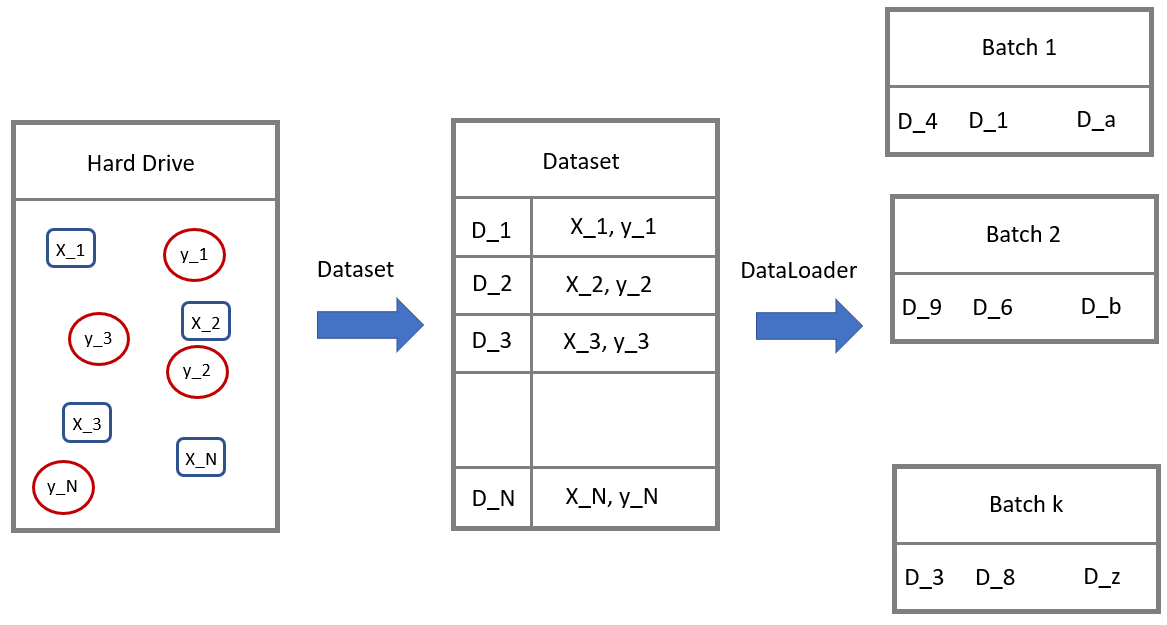
\includegraphics[width=1.0\textwidth,height=1.0\textheight,keepaspectratio]{images/dataloaders.png}
\end{figure}
\end{frame} 